\documentclass{article}
\usepackage[a4paper, hmargin={2.5cm, 2.5cm}, vmargin={2.5cm, 2.5cm}]{geometry}
\usepackage[utf8]{inputenc}
\usepackage[english]{babel}
\usepackage{amsmath,amssymb,graphicx}
\usepackage{cleveref}
\usepackage{hyperref}

\usepackage{mathtools}
\usepackage{fancyhdr}
\usepackage{lastpage}
\usepackage{geometry}
\usepackage{ulem}
\usepackage{gauss}
\usepackage{graphicx}
\usepackage{pdfpages}
\usepackage{hyperref}
\usepackage{cleveref}
\usepackage{wrapfig}
\usepackage{morefloats}
\usepackage{upquote}


%%%%%% COLORS %%%%%%%%

\usepackage{xcolor}
\definecolor{red1}{rgb}{0.7, 0.0, 0.3}
\definecolor{red2}{rgb}{0.5, 0.0, 0.5}
\definecolor{red3}{rgb}{0.3, 0.0, 0.7}

%two definitions of the color grey
\usepackage{color}
\definecolor{listinggray}{gray}{0.9}
%\definecolor{lbcolor}{rgb}{0.9,0.9,0.9}

\usepackage{listings}
\lstset{
	language=,
	literate=
		{æ}{{\ae}}1
		{ø}{{\o}}1
		{å}{{\aa}}1
		{Æ}{{\AE}}1
		{Ø}{{\O}}1
		{Å}{{\AA}}1
		{'}{{'}}1,
	backgroundcolor=\color{listinggray},
	tabsize=3,
	rulecolor=,
	basicstyle=\scriptsize,
	upquote=true,
	aboveskip={1.5\baselineskip},
	columns=fixed,
	showstringspaces=false,
	extendedchars=true,
	breaklines=true,
	prebreak =\raisebox{0ex}[0ex][0ex]{\ensuremath{\hookleftarrow}},
	frame=single,
	showtabs=false,
	showspaces=false,
	showstringspaces=false,
	identifierstyle=\ttfamily,
	keywordstyle=\color[rgb]{0,0,1},
	commentstyle=\color[rgb]{0.133,0.545,0.133},
	stringstyle=\color[rgb]{0.627,0.126,0.941},
}

\lstset{moredelim=[s][\color{gray}]{(*}{*)}}
\lstset{morecomment=[l][\color{gray}]{##}}
\lstset{moredelim=[s][\color{green!50!brown}]{"}{"}}
\lstset{moredelim=[s][\color{green!50!brown}]{'}{'}}
\lstset{moredelim=[s][\color{gray}]{/*}{*/}}

\lstset{literate=
	{0}{{{\color{violet}{0}}}}1
	{1}{{{\color{violet}{1}}}}1
	{2}{{{\color{violet}{2}}}}1
	{3}{{{\color{violet}{3}}}}1
	{4}{{{\color{violet}{4}}}}1
	{5}{{{\color{violet}{5}}}}1
	{6}{{{\color{violet}{6}}}}1
	{7}{{{\color{violet}{7}}}}1
	{8}{{{\color{violet}{8}}}}1
	{9}{{{\color{violet}{9}}}}1
	{?}{{{\color{orange}{?}}}}1
}

\lstset{emph={for, in, if, elif, else, return, def, print}, emphstyle={\color{blue}},,
        emph={[3]std}, emphstyle={[3]\color{green}}}

\lstset{emph={True, False}, emphstyle={\color{violet}},,
        emph={[3]std}, emphstyle={[3]\color{green}}}

%captions on listings
\usepackage[center,font=small,labelfont=bf,textfont=it]{caption}

\title{Insert Assignment Title Here\\02807 Computational Tools for Big Data}
\author{Anonymous authors}
\date{26th October 2015}

\setlength\parindent{0pt}		% noindent through whole document
\usepackage[parfill]{parskip}	% extra linebreak on new paragraph

\begin{document}

\maketitle

\section{Exercide 5}
\label{sec:Exercide 5}

\subsection{Exercise 5.1}
\label{sub:Exercise 5.1}

\textbf{SQLite}:

We run the following python code in order to find all tables in the database:

\begin{lstlisting}
self.conn = sqlite3.connect(os.path.dirname(__file__) + '/../data/northwind.db')
self.conn.text_factory = str
c = self.conn.cursor()
tables = c.execute("SELECT * FROM sqlite_master WHERE type='table';").fetchall()
self.conn.close()
\end{lstlisting}

Printing $tables$ yields the following result:

\begin{lstlisting}
['Categories',
 'sqlite_sequence',
 'CustomerCustomerDemo',
 'CustomerDemographics',
 'Customers',
 'Employees',
 'EmployeeTerritories',
 'Order Details',
 'Orders',
 'Products',
 'Regions',
 'Shippers',
 'Suppliers',
 'Territories']
\end{lstlisting}

\newpage

\textbf{MongoDB}:

We run the following python code in order to find all customers who reside in the city of Berline.

\begin{lstlisting}
self.client = MongoClient()
self.db = self.client['Northwind']
documents = []
    for doc in self.db['customers'].find({'City': 'Berlin'}):
        documents += [doc]
\end{lstlisting}

If we print $documents$ we get the following result.

\begin{lstlisting}
[{u'Address': u'Obere Str. 57',
  u'City': u'Berlin',
  u'CompanyName': u'Alfreds Futterkiste',
  u'ContactName': u'Maria Anders',
  u'ContactTitle': u'Sales Representative',
  u'Country': u'Germany',
  u'CustomerID': u'ALFKI',
  u'Fax': u'030-0076545',
  u'Phone': u'030-0074321',
  u'PostalCode': 12209,
  u'Region': u'NULL',
  u'_id': ObjectId('5626242620dcd23954bcb018')}]
\end{lstlisting}

\subsection{Exercise 5.2}
\label{sub:Exercise 5.2}

In order to help with using MongoDB code in exercise 5 we have implemented the following helper class:

\begin{lstlisting}
class Mongodb(object):
    def __init__(self, dbname):
        self.client = MongoClient()
        self.db = self.client[dbname]

    def group_by(self, obj, key, condition, reduce_function, initial, finalize=None):
        documents = []
        for doc in self.db[obj].group(key=key, condition=condition, reduce=reduce_function, initial=initial, finalize=finalize):
            documents += [doc]
        return documents

    def find_all(self, obj):
        documents = []
        for doc in self.db[obj].find():
            documents += [doc]
        return documents

    def find_by(self, obj, selector):
        documents = []
        for doc in self.db[obj].find(selector):
            documents += [doc]
        return documents

    def join(self, collection1, obj, fk1, fk2):
        return filter(
            lambda x: True if x[fk1] == obj[fk2] else False,
            collection1
        )

    def join_in(self, collection1, collection2, fk):
        return filter(
            lambda x: True if x[fk] in collection2 else False,
            collection1
        )
\end{lstlisting}

\newpage

The actual code we use to solve exercise 5.2 looks as follows:

\begin{lstlisting}
db = Mongodb('Northwind')

orders = db.find_by('orders', {'CustomerID': 'ALFKI'})

order_details = db.find_by(
    'order-details', {
        'OrderID': {
            '$in': map(lambda x: x['OrderID'], orders)
        }
    }
)

products = db.find_by(
    'products', {
        'ProductID': {
            '$in': map(lambda x: x['ProductID'], order_details)
        }
    }
)


#  excercise 5.2
def excercise5_2():
    for order in orders:
        print 'Order ID:' + str(order['OrderID'])
        pprint(
            map(
                lambda y: y['ProductName'],
                db.join_in(
                    products,
                    map(
                        lambda x: x['ProductID'],
                        db.join(order_details, order, 'OrderID', 'OrderID')
                    ),
                    'ProductID'
                )
            )
        )
\end{lstlisting}

If we run the function $excercise5_2$ we get the following output:

\begin{lstlisting}
Order ID:10643
[u'R\xf6ssle Sauerkraut', u'Chartreuse verte', u'Spegesild']
Order ID:10692
[u'Vegie-spread']
Order ID:10702
[u'Aniseed Syrup', u'Lakkalik\xf6\xf6ri']
Order ID:10835
[u'Raclette Courdavault', u'Original Frankfurter gr\xfcne So\xdfe']
Order ID:10952
[u"Grandma's Boysenberry Spread", u'R\xf6ssle Sauerkraut']
Order ID:11011
[u'Escargots de Bourgogne', u'Flotemysost']
\end{lstlisting}

\subsection{Exercise 5.3}
\label{sub:Exercise 5.3}

Given the same helper class we use the following function to solve exercise 5.3:

\begin{lstlisting}
def excercise5_3():
    for order in orders:
        order_products = map(
            lambda y: y['ProductName'],
            db.join_in(
                products,
                map(
                    lambda x: x['ProductID'],
                    db.join(order_details, order, 'OrderID', 'OrderID')
                ),
                'ProductID'
            )
        )

        if len(order_products) > 1:
            print 'Order ID:' + str(order['OrderID'])
            pprint(order_products)
\end{lstlisting}

Running the function $excercise5_3$ yields the followinh result:

\begin{lstlisting}
Order ID:10643
[u'R\xf6ssle Sauerkraut', u'Chartreuse verte', u'Spegesild']
Order ID:10702
[u'Aniseed Syrup', u'Lakkalik\xf6\xf6ri']
Order ID:10835
[u'Raclette Courdavault', u'Original Frankfurter gr\xfcne So\xdfe']
Order ID:10952
[u"Grandma's Boysenberry Spread", u'R\xf6ssle Sauerkraut']
Order ID:11011
[u'Escargots de Bourgogne', u'Flotemysost']
\end{lstlisting}

\subsection{Exercise 5.4}
\label{sub:Exercise 5.4}

Given the same prequisite helper class, we use the following function to solve exercise 5.4:

\begin{lstlisting}
def excercise5_4():
    order_details = db.find_by('order-details', {'ProductID': 7})

    orders = db.find_by('orders', {
        'OrderID': {
            '$in': map(lambda x: x['OrderID'], order_details)
        }
    })

    customers = db.find_by('customers', {
        'CustomerID': {
            '$in': map(lambda x: x['CustomerID'], orders)
        }
    })

    return customers
\end{lstlisting}

Running the function $excercise5_4$ and printing the result yields the following:

\begin{lstlisting}
Total number of customers: 20
[u'Laurence Lebihan',
 u'Elizabeth Lincoln',
 u'Victoria Ashworth',
 u'Roland Mendel',
 u'Martine Ranc\xe9',
 u'Maria Larsson',
 u'Andr\xe9 Fonseca',
 u'Daniel Tonini',
 u'Carlos Gonz\xe1lez',
 u'Yvonne Moncada',
 u'Ann Devon',
 u'Henriette Pfalzheim',
 u'Horst Kloss',
 u'Paula Wilson',
 u'Maurizio Moroni',
 u'Jonas Bergulfsen',
 u'Jose Pavarotti',
 u'Art Braunschweiger',
 u'Palle Ibsen',
 u'Mary Saveley']
\end{lstlisting}

\newpage

\subsection{Exercise 5.5}
\label{sub:Exercise 5.5}

In order to solve exercise 5.5 we reuse the function from exercise 5.4:

\begin{lstlisting}
def excercise5_5():
    customers = excercise5_4()

    orders = db.find_by('orders', {
        'CustomerID': {
            '$in': map(lambda x: x['CustomerID'], customers)
        }
    })

    order_details = db.find_by('order-details', {
        'OrderID': {
            '$in': map(lambda x: x['OrderID'], orders)
        }
    })

    products = db.find_by('products', {
        'ProductID': {
            '$in': map(lambda x: x['ProductID'], order_details),
            '$not': re.compile("7")
        }
    })

    pprint(len(products))
    pprint(map(lambda x: x['ProductName'], products))
\end{lstlisting}

Running the function $excercise5_5$ yields the following result:

\begin{lstlisting}
Product count: 76
[u'Chai',
 u'Aniseed Syrup',
 u"Chef Anton's Cajun Seasoning",
 u"Chef Anton's Gumbo Mix",
 u"Grandma's Boysenberry Spread",
 u'Chang',
 u"Uncle Bob's Organic Dried Pears",
 u'Mishi Kobe Niku',
 u'Ikura',
 u'Northwoods Cranberry Sauce',
 u'Queso Cabrales',
 u'Queso Manchego La Pastora',
 u'Konbu',
 u'Tofu',
 u'Genen Shouyu',
 u'Pavlova',
 u'Alice Mutton',
 u'Carnarvon Tigers',
 u'Teatime Chocolate Biscuits',
 u"Sir Rodney's Marmalade",
 u"Sir Rodney's Scones",
 u"Gustaf's Kn\xe4ckebr\xf6d",
 u'Tunnbr\xf6d',
 u'Guaran\xe1 Fant\xe1stica',
 u'Gumb\xe4r Gummib\xe4rchen',
 u'NuNuCa Nu\xdf-Nougat-Creme',
 u'Schoggi Schokolade',
 u'R\xf6ssle Sauerkraut',
 u'Th\xfcringer Rostbratwurst',
 u'Nord-Ost Matjeshering',
 u'Gorgonzola Telino',
 u'Mascarpone Fabioli',
 u'Geitost',
 u'Sasquatch Ale',
 u'Steeleye Stout',
 u'Inlagd Sill',
 u'Gravad lax',
 u'C\xf4te de Blaye',
 u'Chartreuse verte',
 u'Boston Crab Meat',
 u"Jack's New England Clam Chowder",
 u'Singaporean Hokkien Fried Mee',
 u'Ipoh Coffee',
 u'Gula Malacca',
 u'Rogede sild',
 u'Spegesild',
 u'Zaanse koeken',
 u'Chocolade',
 u'Maxilaku',
 u'Valkoinen suklaa',
 u'Manjimup Dried Apples',
 u'Filo Mix',
 u'Perth Pasties',
 u'Tourti\xe8re',
 u'P\xe2t\xe9 chinois',
 u'Gnocchi di nonna Alice',
 u'Ravioli Angelo',
 u'Escargots de Bourgogne',
 u'Raclette Courdavault',
 u'Camembert Pierrot',
 u"Sirop d'\xe9rable",
 u'Tarte au sucre',
 u'Vegie-spread',
 u'Wimmers gute Semmelkn\xf6del',
 u'Louisiana Fiery Hot Pepper Sauce',
 u'Louisiana Hot Spiced Okra',
 u'Scottish Longbreads',
 u'Gudbrandsdalsost',
 u'Outback Lager',
 u'Flotemysost',
 u'Mozzarella di Giovanni',
 u'R\xf6d Kaviar',
 u'Longlife Tofu',
 u'Rh\xf6nbr\xe4u Klosterbier',
 u'Lakkalik\xf6\xf6ri',
 u'Original Frankfurter gr\xfcne So\xdfe']
\end{lstlisting}

\subsection{Exercise 5.6}
\label{sub:Exercise 5.6}

To solve exercise 5.6 we use the following function:

\begin{lstlisting}
def excercise5_6():
    customers = excercise5_4()

    orders = db.find_by('orders', {
        'CustomerID': {
            '$in': map(lambda x: x['CustomerID'], customers)
        }
    })

    gb = db.group_by(
        'order-details',
        key={'ProductID': 1},
        condition={
            'OrderID': {
                '$in': map(lambda x: x['OrderID'], orders)
            }
        },
        reduce_function='function (current, result) { result.total += current.Quantity; }',
        initial={'total': 0}
    )

    gb.sort(key=lambda x: x['total'], reverse=True)

    pprint(gb[0])

    product = db.find_by('products', {
        'ProductID': gb[0]['ProductID']
    })

    pprint(product)
\end{lstlisting}

Running the function $exercise5_6$ yields the following result:

\begin{lstlisting}
{u'ProductID': 60.0, u'total': 769.0}
[{u'CategoryID': 4,
  u'Discontinued': 0,
  u'ProductID': 60,
  u'ProductName': u'Camembert Pierrot',
  u'QuantityPerUnit': u'15 - 300 g rounds',
  u'ReorderLevel': 0,
  u'SupplierID': 28,
  u'UnitPrice': 34.0,
  u'UnitsInStock': 19,
  u'UnitsOnOrder': 0,
  u'_id': ObjectId('5626242620dcd23954bcbc88')}]
\end{lstlisting}

\section{Exercise 6}
\label{sec:Exercise 6}

\subsection{Exercise 6.1}
\label{sub:Exercise 6.1}

Here you can see we have created a Graph Story account and generated a database:

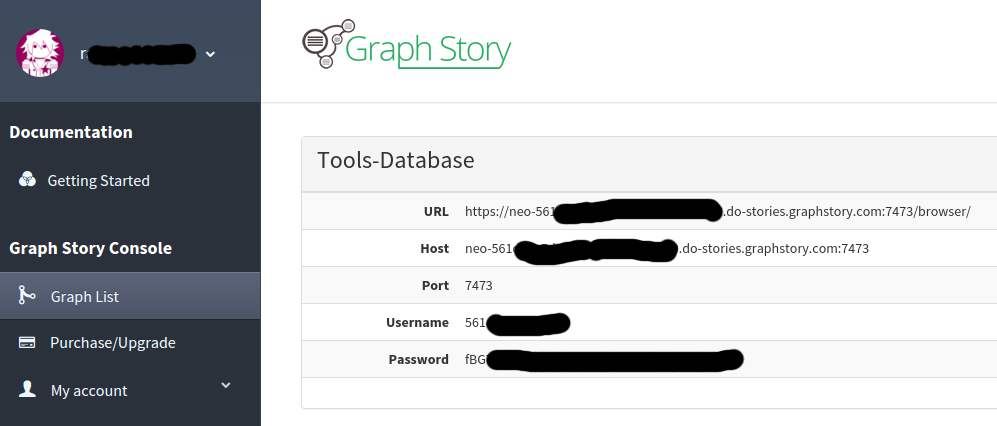
\includegraphics[scale=0.45]{graph_story.png}

Then we removed all data from the database:

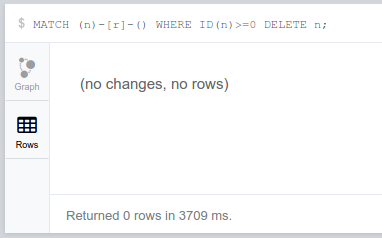
\includegraphics[scale=0.5]{delete_all.png}

Lastly, we loaded all the data into the database, using the given code.
I've chosen to only include the output of the last line of code, which should be
enough proof that we have done them all.

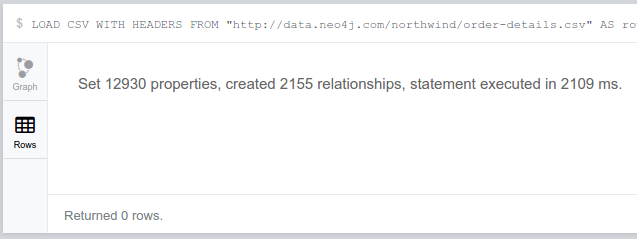
\includegraphics[scale=0.5]{insert_data.png}

\subsection{Exercise 6.2}
\label{sub:Exercise 6.2}

Using the following query, we are able to find all orders for the customer with
customerID 'ALFKI', including the products in those orders.

\begin{lstlisting}
MATCH (customer {customerID:'ALFKI'})--(orders) RETURN orders
\end{lstlisting}

This returns the following graph from the database:

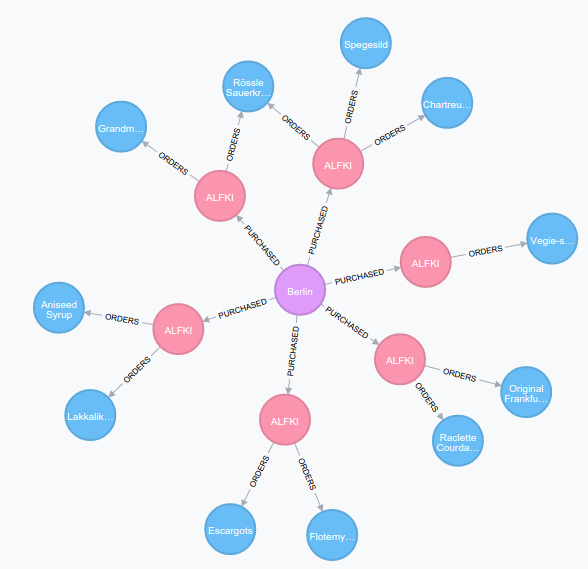
\includegraphics[scale=0.5]{6_2.png}

Here, the purple circle is the customer, the red circles are orders, and the blue
circles are the products.


\subsection{Exercise 6.3}
\label{sub:Exercise 6.3}

Using the following query, we are able to find all orders for the customer with
customerID 'ALFKI', including only the orders with at least 2 products.

\begin{lstlisting}
MATCH (customer {customerID:'ALFKI'})--(order)
MATCH p=(order)--(X)
WITH order as order, count(p) as paths
WHERE paths > 2
RETURN order
\end{lstlisting}

This returns the following graph from the database:

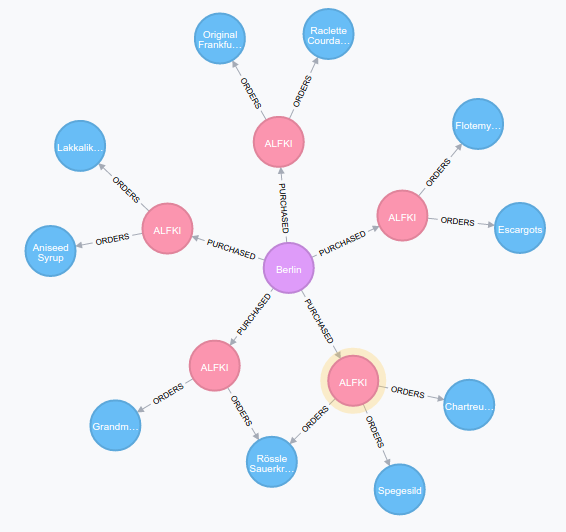
\includegraphics[scale=0.5]{6_3.png}

\subsection{Exercise 6.4}
\label{sub:Exercise 6.4}



\end{document}
